\subsubsection{SAS URL Generation}

The generation of a secure, temporary link (SAS URL) to the receipts stored in Azure Blob Storage is handled by the \texttt{BlobStorageService} class. This class uses the Azure Storage SDK to create a short-lived URL with read-only permissions. This URL is then sent to the external AI service, allowing secure access to the file and avoiding permanent public access without requiring a complex credential strategy. 

At the same time, the client (frontend) also requests the URL to display the file associated with the expense to its owner. The code implementation for generating the SAS URL is presented in Figure~\ref{fig:sas-url-generation}.


\begin{figure}[H]
    \centering
    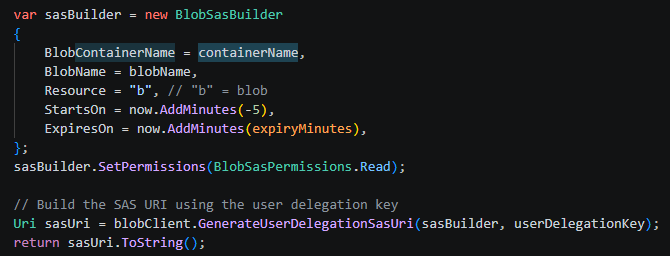
\includegraphics[width=0.7\textwidth]{Images/Implementation/SASURLGeneration.png}
    \caption[SAS URL generation in BlobStorageService.cs]
    {SAS URL generation in \texttt{BlobStorageService.cs}. [Own creation]}
    \label{fig:sas-url-generation}
\end{figure}